\documentclass[handout,a4paper,slidestop,xcolor=pst,blue]{beamer}

\usepackage{beamerthemesplit}
\usepackage[utf8]{inputenc}
\usepackage[spanish]{babel}
\usepackage{graphicx}
\usepackage{pstricks} % PSTricks package
\usepackage{setspace}
\usepackage{multirow}
\usepackage{listings}
\usepackage{pgfpages}
\usepackage{hyperref}
\usepackage{etoolbox}
\usepackage{epstopdf}

\makeatletter
\patchcmd{\beamer@sectionintoc}{\vskip1.5em}{\vskip0.5em}{}{}
\makeatother

\setbeamercovered{dynamic}
\setcounter{tocdepth}{2}
\setbeamercolor{frametitle}{fg=black,bg=white}
\setbeamercolor{section in toc shaded}{fg=black}
\setbeamercolor{section in toc}{fg=red}
\setbeamercolor{subsection in toc shaded}{fg=black}
\setbeamercolor{subsection in toc}{fg=red}
\setbeamerfont{section in toc}{size=\small}
\setbeamerfont{subsection in toc}{size=\small}
\setbeamertemplate{section in toc shaded}[default][99]
\setbeamertemplate{subsection in toc shaded}[default][99]

\AtBeginSection[]
{\begin{frame}[c]
  \frametitle{Índice}
	\tableofcontents[currentsection,
        sectionstyle=show/shaded,
        subsectionstyle=hide]
\end{frame}}

\AtBeginSubsection[]
{\begin{frame}[c]
	\frametitle{Índice}
	\tableofcontents[
  		currentsection,
  		sectionstyle=shaded/shaded,
  		currentsubsection,
  		subsectionstyle=show/shaded/hide
		]
\end{frame}}

\setbeamercolor{frametitle}{fg=black,bg=white}

\setbeamertemplate{frametitle}{
	\begin{centering}
		\insertframetitle
		\par
	\end{centering}
}

\usetheme[secheader]{Boadilla}


\title[Arquitecturas Sw]{Arquitecturas Software}

\author[Pablo S\'{a}nchez]{\alert{Pablo S\'{a}nchez}}

\institute[I2E]{
           Grupo de Ingenier{\'i}a del Software y Tiempo Real \\
		   Dpto. Ingenier{\'i}a Inform{\'a}tica y Electr{\'o}nica \\
		   Universidad de Cantabria \\
		   Santander (Cantabria, España) \\
		   p.sanchez@unican.es
}

\date{}

\begin{document}

\begin{frame}[c]
	\titlepage
	\begin{columns}
		\column{0.50\linewidth}
			\centering
    		
\includegraphics[width=.28\textwidth,keepaspectratio=true]{images/istr.eps}
		\column{0.50\linewidth}
			\centering
			
\includegraphics[width=.25\textwidth,keepaspectratio=true]{images/uc.eps}
	\end{columns}
\end{frame}

\section{Introducción}

\subsection{Objetivos}

\begin{frame}[c]
	\frametitle{Objetivos}
	\begin{enumerate}[<+->]
		\item Comprender el concepto y utilidad de las \emph{arquitecturas sw}.
		\item Comprender el concepto de \emph{componente} y \emph{conector}.
        \item Comprender para qué sirve un lenguaje de \emph{descripción arquitectónica}.
        \item Comprender el concepto de \emph{vista arquitectónica}.
		\item Conocer y comprender los principales tipos de \emph{vistas arquitectónicas}.
		\item Conocer qué contienen las vistas arquitectónicas de los principales modelos de referencia como \emph{TOGAF}.
    \end{enumerate}
\end{frame}

\begin{frame}[c]
    \frametitle{Objetivos}
    \begin{enumerate}[<+->]
        \setcounter{enumi}{6}
        \item Conocer algunos patrones arquitectónicos de dominios diferentes a los sistemas empresariales.
        \item Comprender cómo funcionan los procesos de diseño de arquitecturas sw y, en especial, \emph{Attribute-Based Architecture Design (AAD)}.
		\item Comprender cómo funcionan las técnicas de análisis de las arquitecturas sw, y en particular, \emph{Architecture Tradeoff Analysis Method (ATAM)}.
	\end{enumerate}
\end{frame}

\subsection{Bibliografía}

\begin{frame}[c]
	\frametitle{Bibliografía}
    \begin{thebibliography}{}
        \bibitem[Taylor et~al., 2009]{taylor:2009x}
        Taylor, R.~N., Medvidovic, N., and Dashofy, E. (2009).
        \newblock {\em {Software Architecture: Foundations, Theory, and Practice}}.
        \newblock Wiley.

        \bibitem[Fowler, 2002]{Fowler2002x}
        Fowler, M. (2002).
        \newblock {\em {Patterns of Enterprise Application Architecture}}.
        \newblock Addison-Wesley Professional.

        \bibitem[Esposito and Saltarello, 2014]{Esposito2014x}
        Esposito, D. and Saltarello, A. (2014).
        \newblock {\em {Microsoft .NET - Architecting Applications for the
          Enterprise}}.
        \newblock 2 edition.
    \end{thebibliography}
\end{frame}

\begin{frame}[c]
	\frametitle{Bibliografía}
    \begin{thebibliography}{}
        \bibitem[Open Group, 2011]{togaf2011x}
        Open Group (2011).
        \newblock TOGAF version 9.1.
        \newblock Standard G116, Open Group Standard.

        \bibitem[Kazman et~al., 2000]{Kazman2000x}
        Kazman, R., Klein, M.~H., and Clements, P.~C. (2000).
        \newblock {ATAM: Method for Architecture Evaluation}.
        \newblock Technical Report CMU/SEI-2000-TR-004, Software Engineering Institute
          (SEI), Carnegie Mellon University (CMU).

        \bibitem[Wojcik et~al., 2006]{Wojcik2006x}
        Wojcik, R., Bachmann, F., Bass, L., Clements, P., Merson, P., Nord, R., and
          Wood, W. (2006).
        \newblock Attribute-Driven Design (ADD), version 2.0.
        \newblock Technical Report CMU/SEI-2006-TR-023, Software Engineering Institute
             (SEI), Carnegie Mellon University (CMU).
    \end{thebibliography}
\end{frame}

\section{Concepto de Arquitectura SW}

\subsection{Motivación}

\begin{frame}[t]
   \frametitle{Fases del Ciclo de Vida Sw}
   \only<1|handout:0>{
	   \rput[lt](0.5,-0.5){
	   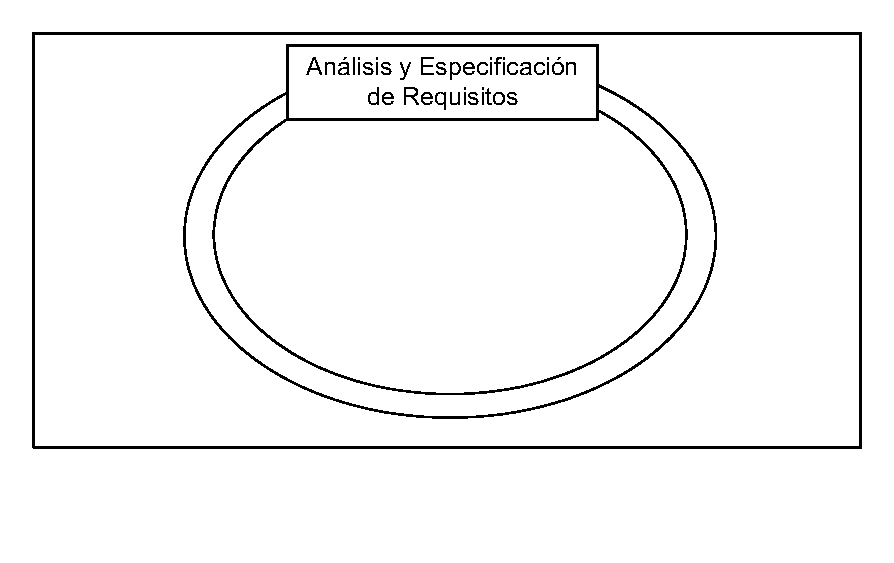
\includegraphics[width=11cm,keepaspectratio=true]{images/ciclosVida/ciclo00.eps}}
   }
   \only<2|handout:1>{
	   \rput[lt](0.5,-0.5){
	   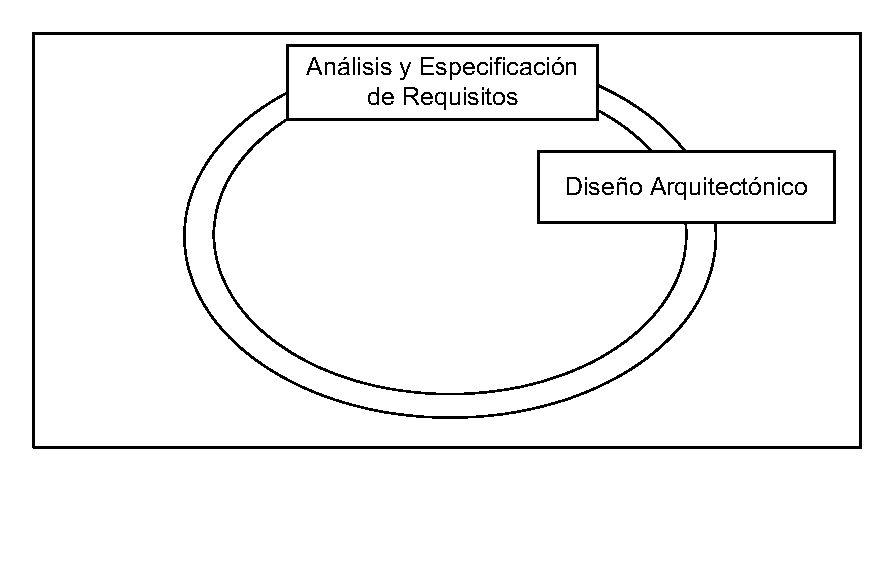
\includegraphics[width=11cm,keepaspectratio=true]{images/ciclosVida/ciclo01.eps}}
   }
\end{frame}

\begin{frame}[t]
	\frametitle{¿Por qué Necesitamos Arquitecturas Sw?}
    \only<1|handout:0>{
	   \rput[lt](0.5,0.25){
        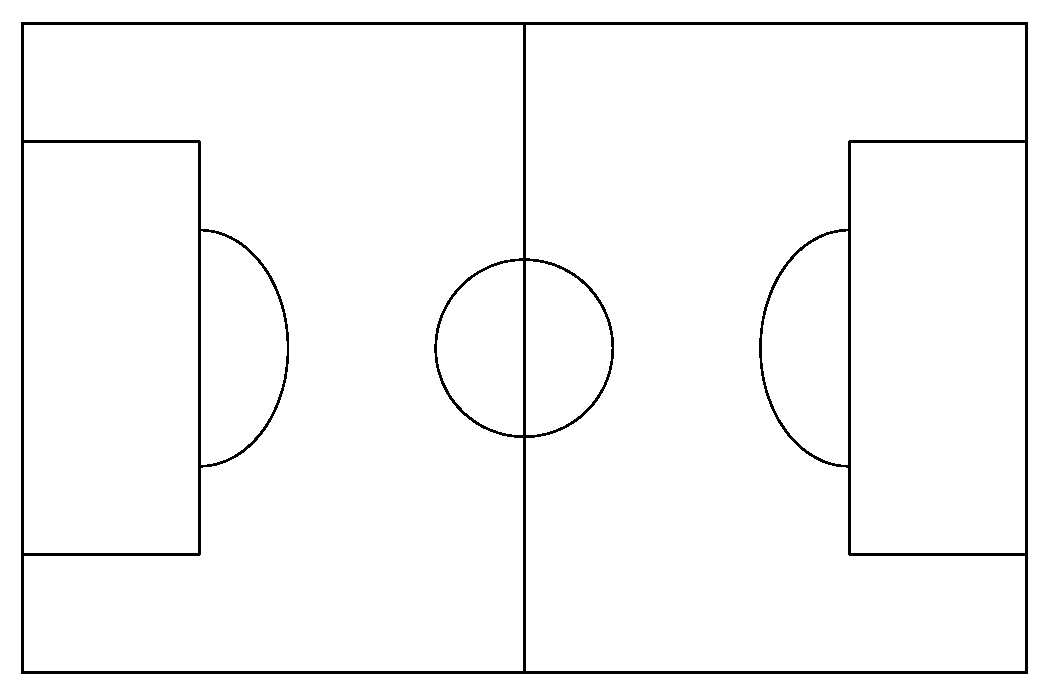
\includegraphics[width=11cm,keepaspectratio=true]{images/introduccion/futbol00.eps}}
	}
	\only<2|handout:0>{
	   \rput[lt](0.5,0.25){
	   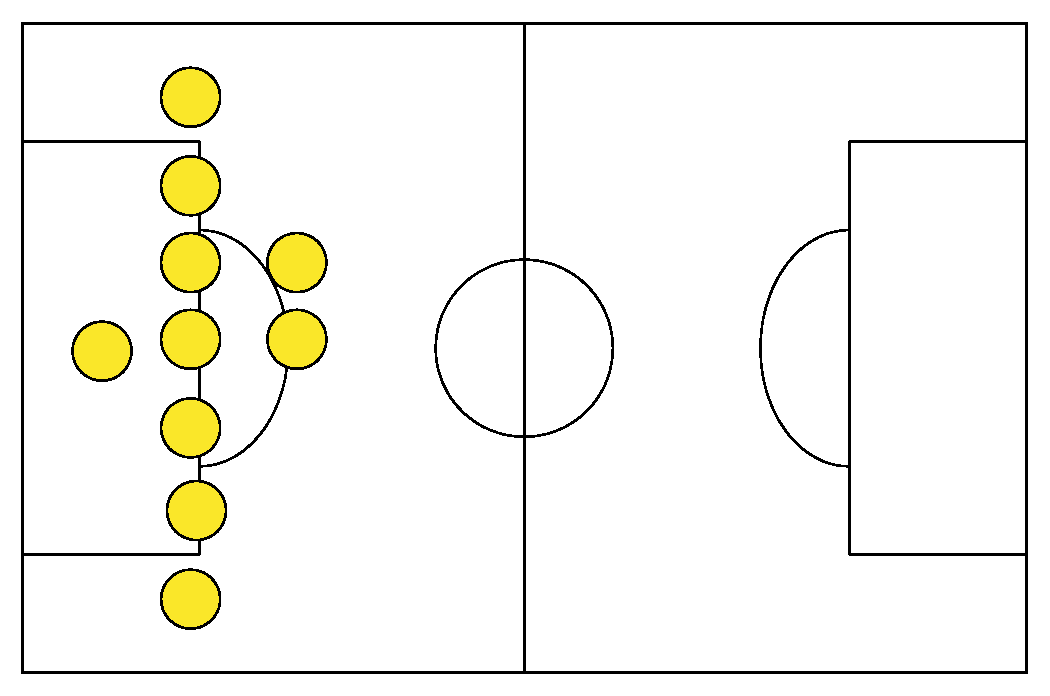
\includegraphics[width=11cm,keepaspectratio=true]{images/introduccion/futbol01.eps}}
	}
	\only<3|handout:0>{
	   \rput[lt](0.5,0.25){
	   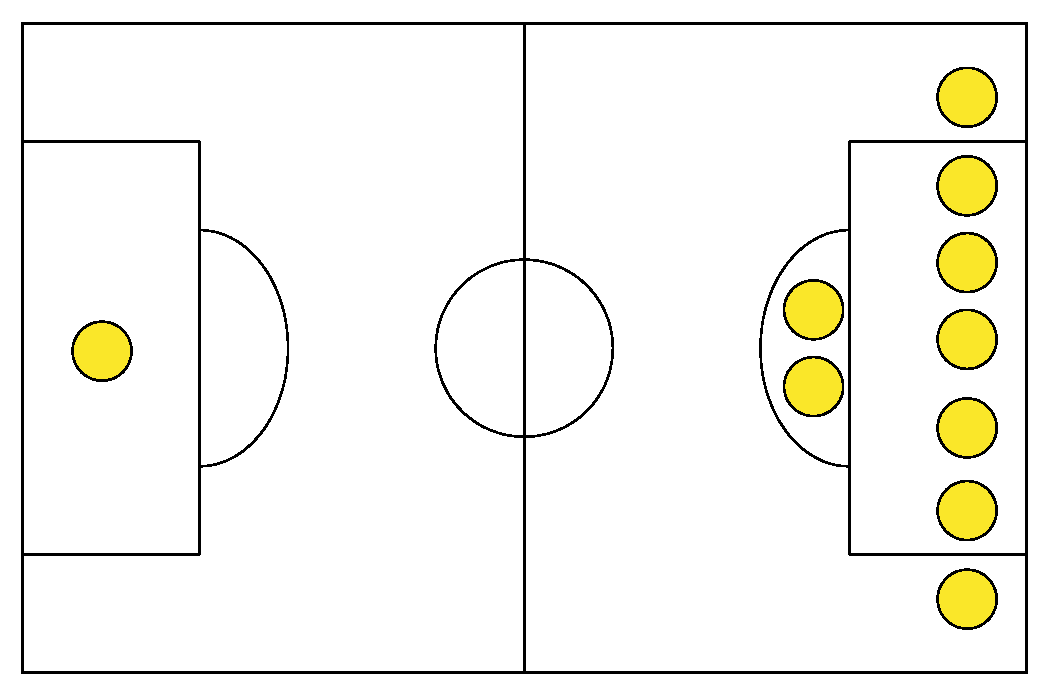
\includegraphics[width=11cm,keepaspectratio=true]{images/introduccion/futbol02.eps}}
	}
	\only<4|handout:1>{
	   \rput[lt](0.5,0.25){
	   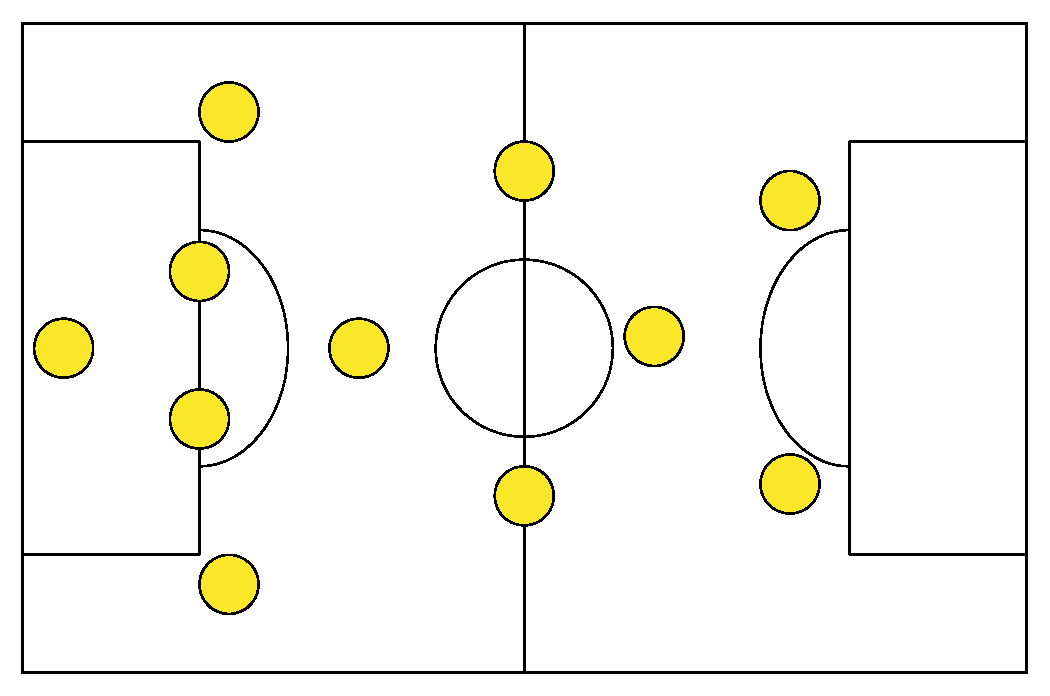
\includegraphics[width=11cm,keepaspectratio=true]{images/introduccion/futbol03.eps}}
	}
	\only<5|handout:0>{
	   \rput[lt](0.5,0.25){
	   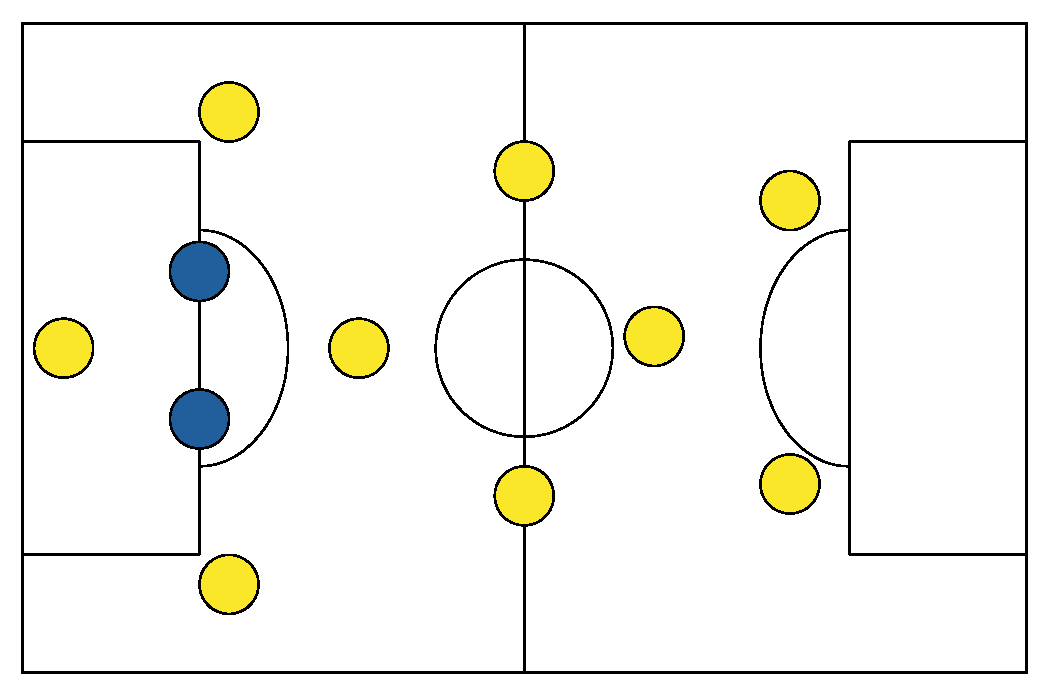
\includegraphics[width=11cm,keepaspectratio=true]{images/introduccion/futbol04.eps}}
	}
	\only<6|handout:0>{
	   \rput[lt](0.5,0.25){
	   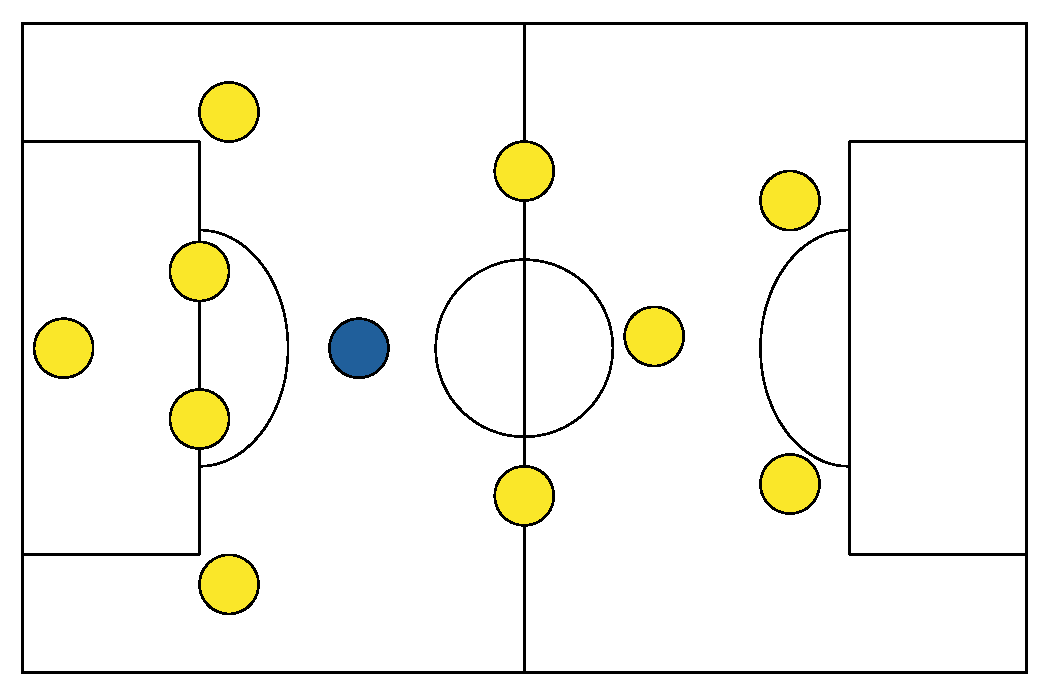
\includegraphics[width=11cm,keepaspectratio=true]{images/introduccion/futbol05.eps}}
	}
	\only<7|handout:0>{
	   \rput[lt](0.5,0.25){
	   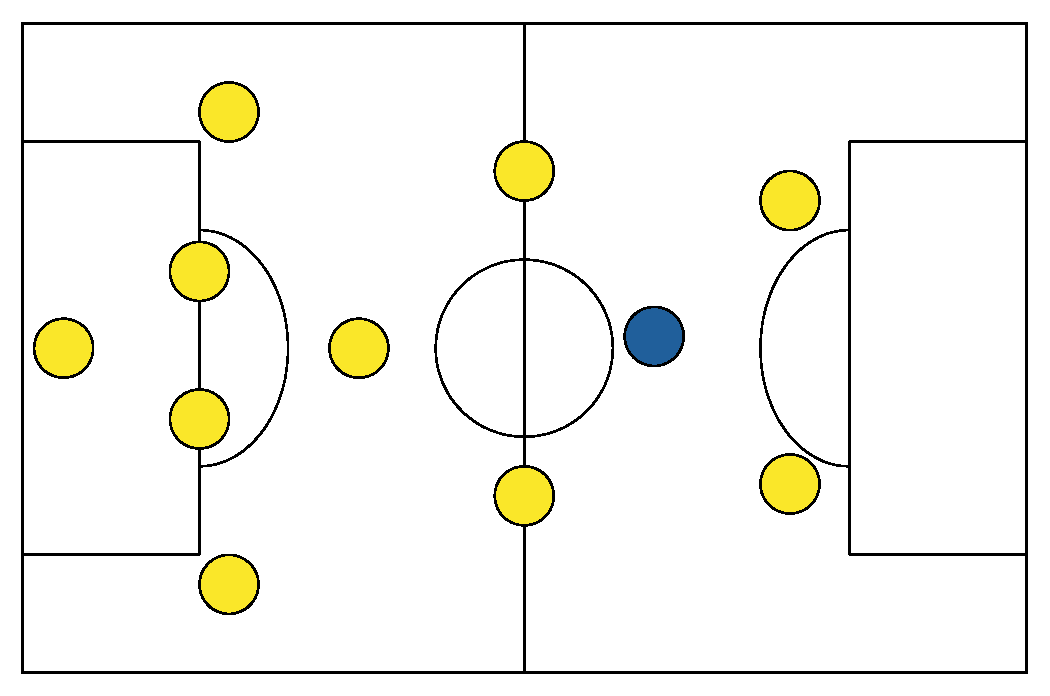
\includegraphics[width=11cm,keepaspectratio=true]{images/introduccion/futbol06.eps}}
	}
	\only<8|handout:0>{
	   \rput[lt](0.5,0.25){
	   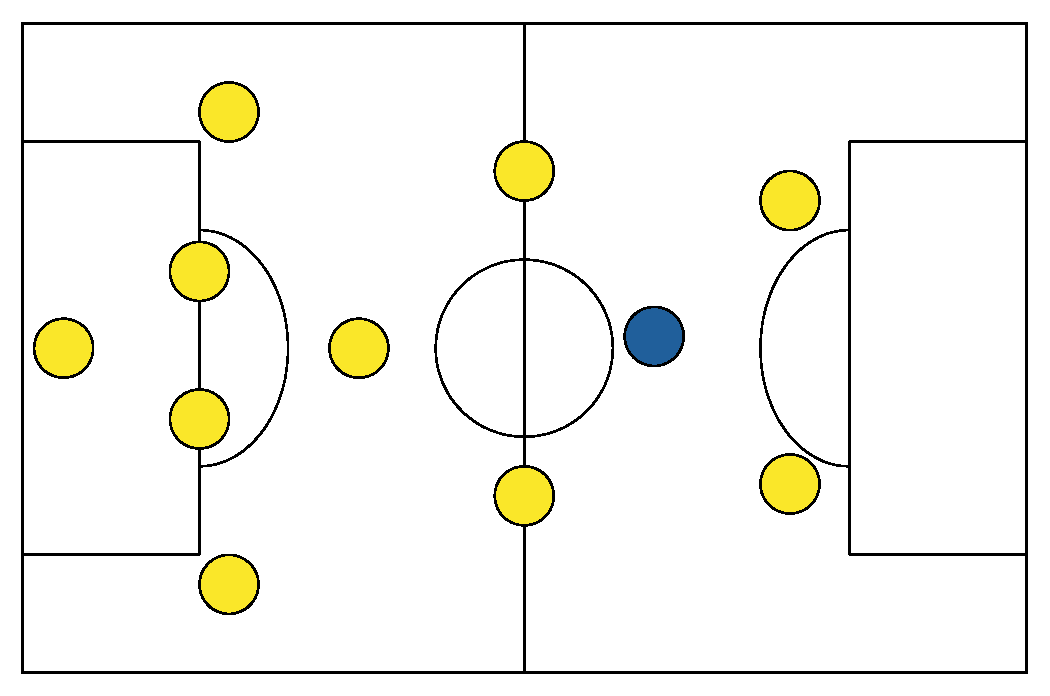
\includegraphics[width=11cm,keepaspectratio=true]{images/introduccion/futbol06.eps}}
	}
\end{frame}

\subsection{Definición de Arquitectura Sw}

\begin{frame}[t]
	\frametitle{Definiciones Arquitectura Sw}
	\begin{block}{Arquitectura Software~\cite{taylor:2009,pohl:2005}}
		La arquitectura de un sistema sw es el conjunto de las principales decisiones de diseño realizadas sobre el sistema. Toda arquitectura sw tiene una \emph{estructura} y una \emph{textura}.
	\end{block}
	\uncover<2->{
		\begin{block}{Textura Arquitectónica~\cite{jazayeri:2000,pohl:2005}}
			La \emph{textura} de un arquitectura sw es el conjunto de reglas que gobiernan el desarrollo y diseño de un sistema software.
		\end{block}
	}
	\uncover<3->{
		\begin{block}{Estructura Arquitectónica~\cite{jazayeri:2000,pohl:2005}}
			La \emph{estructura} de una arquitectura sw es la descomposición de un sistema sw en sus partes principales y las relaciones entre dichas partes.
		\end{block}
	}
\end{frame}

\begin{frame}[c]
	\frametitle{Ventajas de la Definición de Arquitecturas Sw}
    %% TODO: Definir una lectura para esto.
    %% Tentative: Unir Sommerville, Taylor. Revisar Fowler y Santarrello
	\begin{enumerate}[<+->]
		\item Analizar y verificar que satisfaga los requisitos funcionales.
		\item Predecir, analizar y controlar el grado de satisfacción de los requisitos no funcionales desde fases tempranas del desarrollo software.
		\item Facilidad de Evolución.
		\item Facilidad de Comunicación.
		\item Mejora el  Cálculo de Costes
		\item Mejora la Planificación del Proyecto.
	\end{enumerate}
\end{frame}

\begin{frame}[t]
	\frametitle{Objetivos de las Arquitecturas Sw}
    %% TODO: Definir una lectura para esto.
    %% Tentative: Unir Sommerville, Taylor. Revisar Fowler y Santarrello
	\begin{block}{Objetivos Arquitecturas Sw}
        Proporcionar representaciones rigurosas de la arquitectura de un sistema sw (estructura + textura) a partir de las cuales se se puedan obtener respuestas precisas a preguntas concretas, y de manera lo más automática posible.
	\end{block}
\end{frame}

\subsection{Definición de Componente y Connector}

\begin{frame}
	\frametitle{Componente Software}
	\begin{block}{Componente Software~\cite{szyperski:2011}}
		Un \emph{componente sw} es una unidad de composición con interfaces definidas contractualmente y dependencias explícitas con el contexto. Un componente software debe poder ser desplegado de forma independiente y estar sujeto a composición por terceras partes.
	\end{block}
	\uncover<2->{
		\begin{block}{Componente Software~\cite{taylor:2009}}
			Un \emph{componente sw} es una entidad arquitectónica que:
			\begin{enumerate}
				\item<3-> Encapsula un subconjunto de la funcionalidad y/o datos de un sistema sw;
				\item<4-> Restringe el acceso a esa funcionalidad o datos mediante interfaces;
				\item<5-> Define explícitamente sus dependencias con respecto al contexto de ejecución que requiere.
			\end{enumerate}
		\end{block}
	}
\end{frame}

\begin{frame}
   \frametitle{Conector Software}
   \begin{block}{Conector~\cite{taylor:2009}}
		Un \emph{conector sw} es un elemento arquitectónico cuya tarea es establecer y regular la comunicación entre componentes sw.
		% Procedure call
		% Shared Data Access
		% Remote Procedure Calls
		% Adaptors
	\end{block}
\end{frame}

\subsection{Vistas Arquitectónicas}

%%========================================================================%%
%% NOTA(Pablo): Del Prologo de "Documenting Software Architectures ..."   %%
%%========================================================================%%
%% La descripción de una vista debe contener:                             %%
%%    - Una representación, gráfica o textual, de los elementos y         %%
%%      relaciones entre elementos de una vista                           %%
%%    - Descripción de cada uno de sus elementos y sus propiedades        %%
%%    - Especificación de las interfaces y comportamiento de cada         %%
%%      elemento                                                          %%
%%    - Descripción de la variabilidad                                    %%
%%    - Justificaciones y decisiones de diseño                            %%
%%    (pag. 15)                                                           %%
%%========================================================================%%

\begin{frame}[c]
	\frametitle{Vista Arquitectónica}
	\begin{block}{Vista Arquitectónica}
		Una \emph{vista arquitectónica} es un conjunto de decisiones de diseño relativas a un mismo propósito.
	\end{block}
	\uncover<2->{
		\begin{block}{Punto de Vista Arquitectónico}
			Un \emph{punto de vista arquitectónico} define el objetivo de una \emph{vista arquitectónica}.
		\end{block}
	}
	%% Página 196 libro de Taylor
	%% Necesidad de la consistencia entre vistas
	%% - Inconsistencias directas
	%% - Refinement Inconsistencies
	%% - Static vs Dinamic
	%% - Dynamic Inconsistencies
\end{frame}

\begin{frame}[c]
	\frametitle{Principales Vistas Arquitectónicas}
	\begin{itemize}
		\item \alert<2->{Componentes y Conectores}.
		\item Implementación.
		\item Despliegue.
		\item Comportamiento.
		\item Concurrencia.
	\end{itemize}
\end{frame}

\subsubsection{Componentes y Conectores}

\begin{frame}[c]
	\frametitle{Componentes y Conectores (Componentes)}
	\begin{center}
		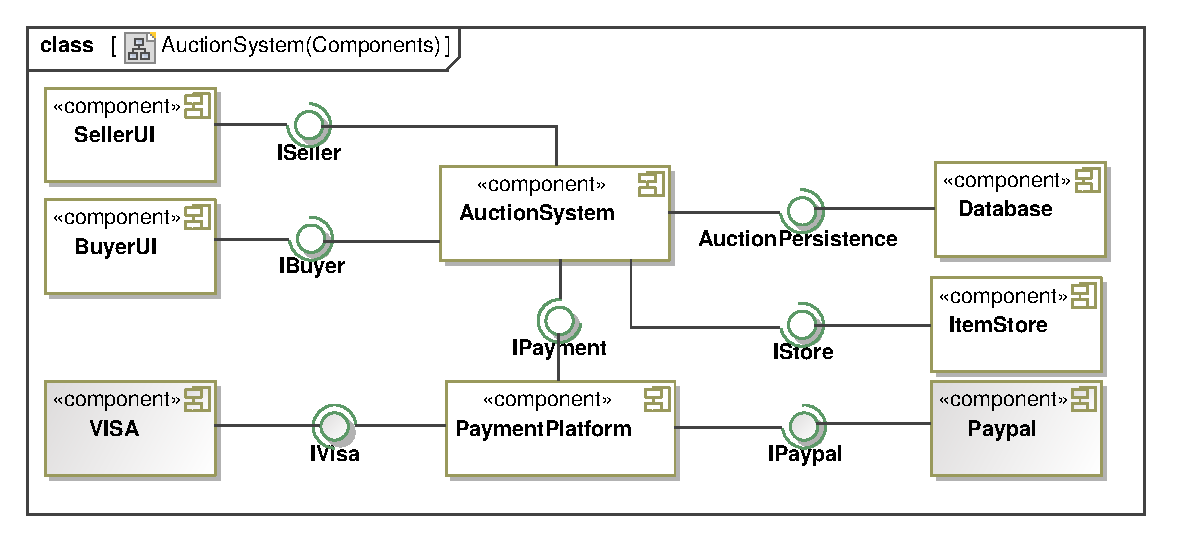
\includegraphics[width=\linewidth]{images/architecturalViews/componentConnector.eps}
	\end{center}
\end{frame}

%\begin{frame}[c]
%	\frametitle{Componentes y Conectores (Instancias)}
%	\begin{center}
%		\includegraphics[width=\linewidth]{images/architecturalViews/componentConnector(Instancias).eps}
%	\end{center}
%\end{frame}
%
%\begin{frame}[c]
%	\frametitle{Componentes y Conectores (Estructura Compuesta)}
%	\begin{center}
%	   \includegraphics[width=\linewidth]{images/architecturalViews/componentConnector(composite).eps}
%	\end{center}
%\end{frame}
%
%\begin{frame}[c]
%	\frametitle{Componentes y Conectores (Interfaces)}
%	\begin{center}
%		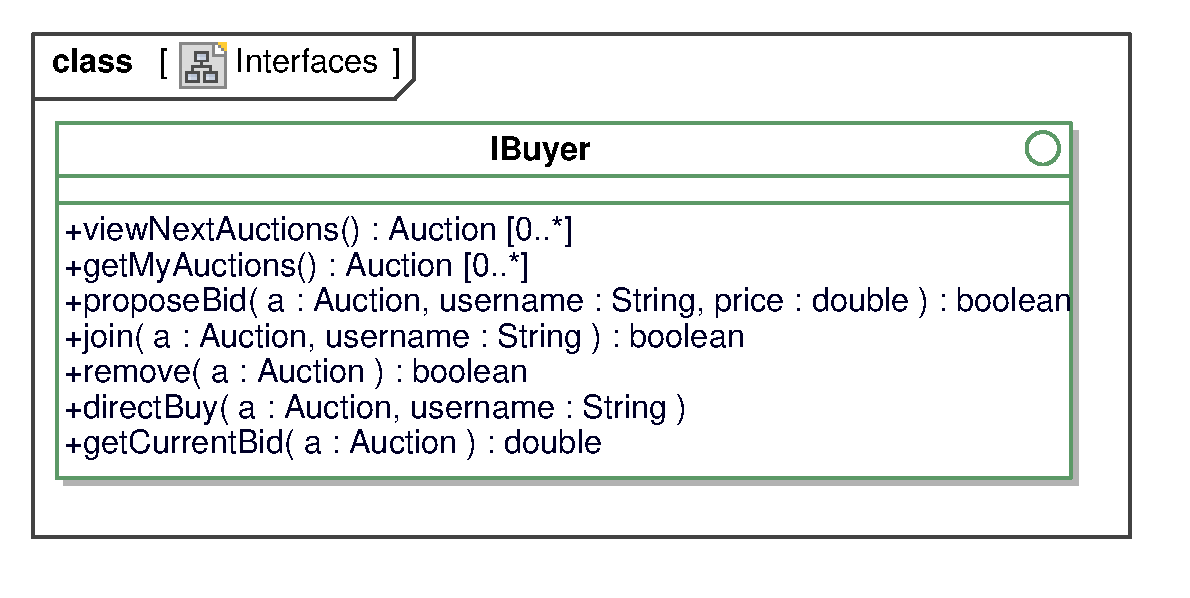
\includegraphics[width=.65\linewidth]{images/architecturalViews/Interfaces.eps}
%	\end{center}
%\end{frame}
%
%\begin{frame}[c]
%	\frametitle{Componentes y Conectores (Tipos de Datos)}
%	\begin{center}
%		\includegraphics[width=.75\linewidth]{images/architecturalViews/Types.eps}
%	\end{center}
%\end{frame}

\subsubsection{Vista de Implementación}

\begin{frame}[c]
	\frametitle{Principales Vistas Arquitectónicas}
	\begin{itemize}
		\item Componentes y Conectores.
        \item \alert{Implementación}.
		\item Despliegue.
		\item Comportamiento.
		\item Concurrencia.
	\end{itemize}
\end{frame}

\begin{frame}[c]
	\frametitle{Vista de Implementación}
	\begin{center}
		\includegraphics[width=\linewidth]{images/architecturalViews/implementation.eps}
	\end{center}
\end{frame}

\subsubsection{Vista de Despliegue}

\begin{frame}[c]
	\frametitle{Principales Vistas Arquitectónicas}
	\begin{itemize}
		\item Componentes y Conectores.
        \item Implementación.
		\item \alert{Despliegue}.
		\item Comportamiento.
		\item Concurrencia.
	\end{itemize}
\end{frame}

\begin{frame}[c]
	\frametitle{Despliegue (Tipos)}
	\begin{center}
		\includegraphics[width=\linewidth]{images/architecturalViews/despliegue(tipos).eps}
	\end{center}
\end{frame}

%\begin{frame}[c]
%	\frametitle{Despliegue (Instancias)}
%	\begin{center}
%		\includegraphics[width=\linewidth]{images/architecturalViews/despliegue(instancias).eps}
%	\end{center}
%\end{frame}

\subsubsection{Vista de Comportamiento}

\begin{frame}[c]
	\frametitle{Principales Vistas Arquitectónicas}
	\begin{itemize}
		\item Componentes y Conectores.
        \item Implementación.
		\item Despliegue.
		\item \alert{Comportamiento}.
		\item Concurrencia.
	\end{itemize}
\end{frame}

%\begin{frame}[c]
%	\frametitle{Protocolo de las Interfaces}
%	\begin{center}
%		\includegraphics[width=.65\linewidth]{images/architecturalViews/protocolo00.eps}
%	\end{center}
%\end{frame}
%
%\begin{frame}[c]
%	\frametitle{Protocolo de las Interfaces}
%	\begin{center}
%		\includegraphics[width=.65\linewidth]{images/architecturalViews/protocolo01.eps}
%	\end{center}
%\end{frame}

\begin{frame}[c]
	\frametitle{Escenario Arquitectónico}
	\begin{center}
		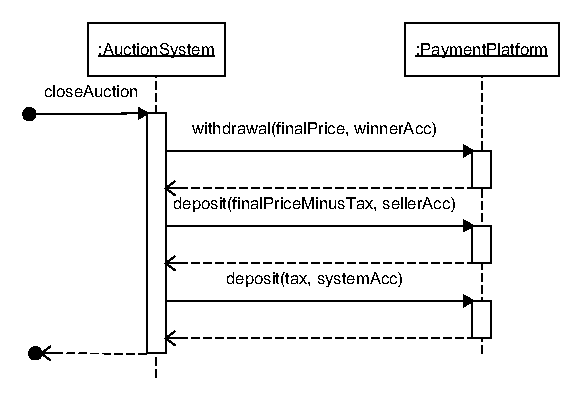
\includegraphics[width=.65\linewidth]{images/architecturalViews/scenario.eps}
	\end{center}
\end{frame}

\subsubsection{Vista de Concurrencia}

\begin{frame}[c]
	\frametitle{Principales Vistas Arquitectónicas}
	\begin{itemize}
		\item Componentes y Conectores.
        \item Implementación.
		\item Despliegue.
		\item Comportamiento.
		\item \alert{Concurrencia}.
	\end{itemize}
\end{frame}

%% TODO: Meter una red de Petri o Similar.

\subsection{Lenguajes de Descripción Arquitectónica}

\begin{frame}[c]
	\frametitle{Lenguajes de Descripción Arquitectónica}
	Lenguaje Natural, \alert<2>{Diseños Ad-hoc}, Darwin, Rapide, Wright, Koala, Weaves, Acme, UML, \alert<2>{AADL}, ADML, xADL, DAOP-ADL, AO-ADL.
\end{frame}

%% Buscar una lista de lenguajes de descripcón arquitectónica y añadirlos a moodle.

\section{Frameworks Arquitectónicos}

\begin{frame}[c]
	\frametitle{Propuestas de Puntos de Vistas Arquitectónicas}
	\begin{enumerate}[<+->]
		\item Modelo 4+1~\cite{krutchen:1995}.
		\item Zachman Framework~\cite{zachman:1987}.
		%% Aplicaciones empresariales
		\item RM-ODP (Reference Model of Open Distributed Processing)~\cite{linington:2011}.
		\item TOGAF.
		\item DoDAF, MoDAF.
	\end{enumerate}
\end{frame}

\subsection{4+1}

\begin{frame}[t]
	\frametitle{Modelo 4+1}
	\only<1|handout:0>{
	   \rput[lt](0.5,0){
	   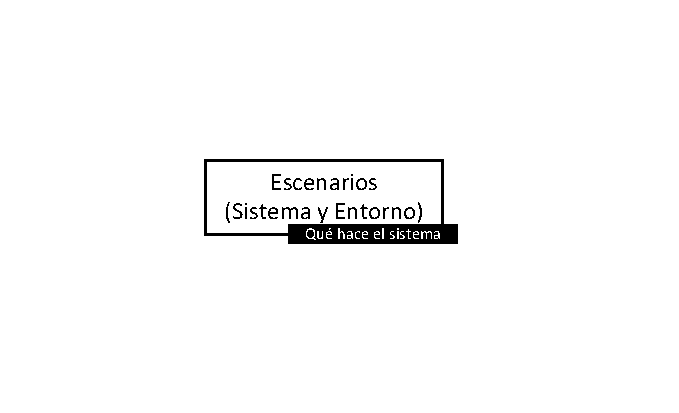
\includegraphics[width=11cm,keepaspectratio=true]{images/architecturalViews/krutchen00.eps}}
	}
	\only<2|handout:0>{
	   \rput[lt](0.5,0){
	   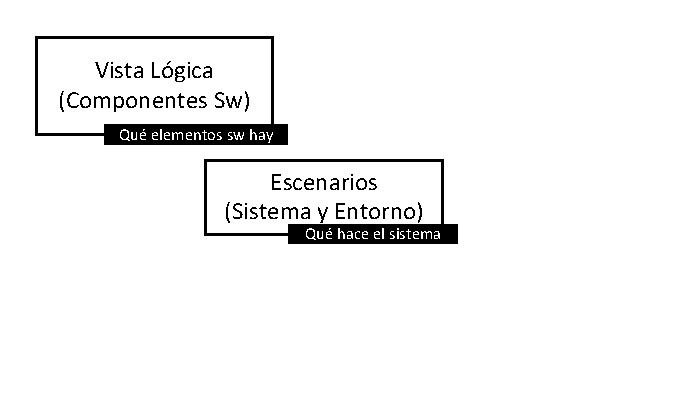
\includegraphics[width=11cm,keepaspectratio=true]{images/architecturalViews/krutchen01.eps}}
	}
	\only<3|handout:0>{
	   \rput[lt](0.5,0){
	   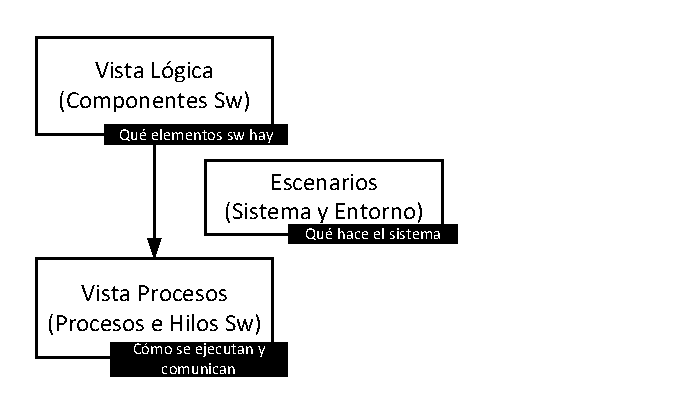
\includegraphics[width=11cm,keepaspectratio=true]{images/architecturalViews/krutchen02.eps}}
	}
	\only<4|handout:0>{
	   \rput[lt](0.5,0){
	   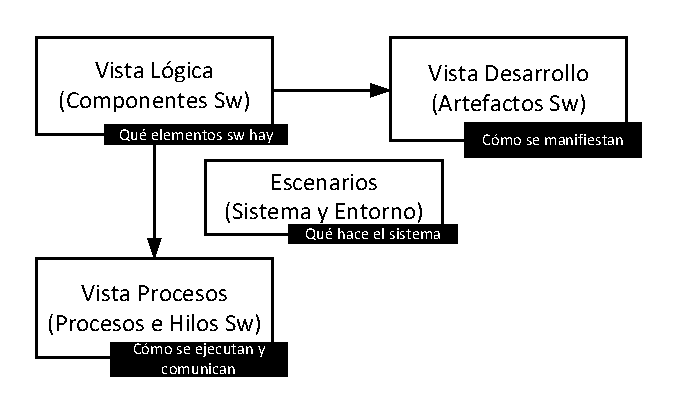
\includegraphics[width=11cm,keepaspectratio=true]{images/architecturalViews/krutchen03.eps}}
	}
	\only<5|handout:1>{
	   \rput[lt](0.5,0){
	   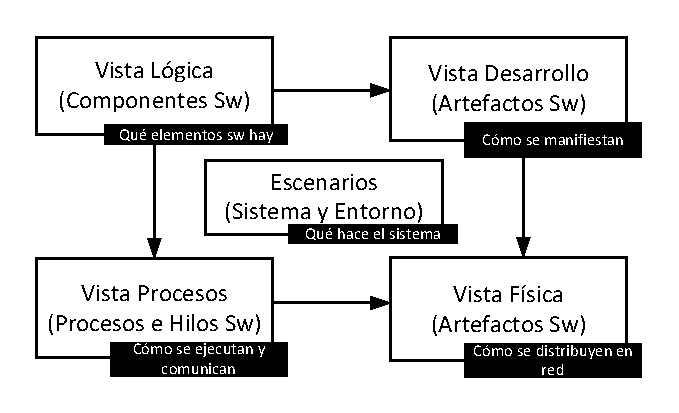
\includegraphics[width=11cm,keepaspectratio=true]{images/architecturalViews/krutchen04.eps}}
	}
\end{frame}

\subsection{RM ODP}

\begin{frame}
	\frametitle{RM ODP}
	%% RM ODP es un estándar para la construcción de sistemas de información que se ejecutan
	%% en un conjunto de nodos hetereogéneos e independientes interconectados por medio de una
	%% red
	\only<1|handout:0>{
	   \rput[lt](0.5,0){
	   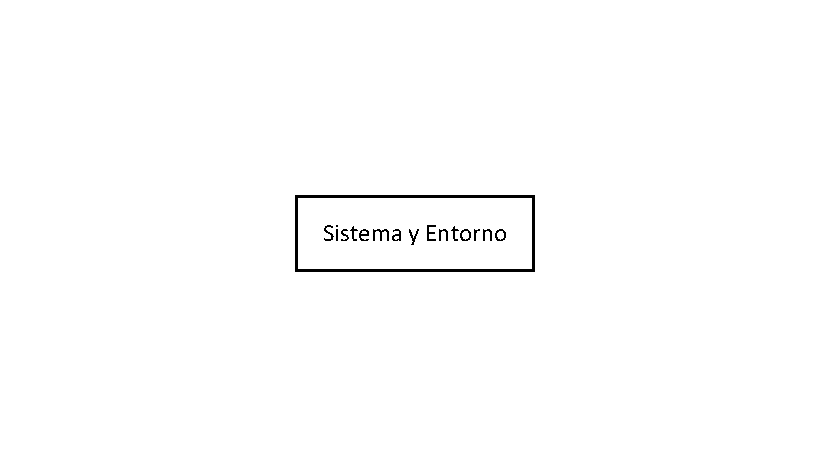
\includegraphics[width=11cm,keepaspectratio=true]{images/architecturalViews/odp00.eps}}
	}
	\only<2|handout:0>{
	   \rput[lt](0.5,0){
	   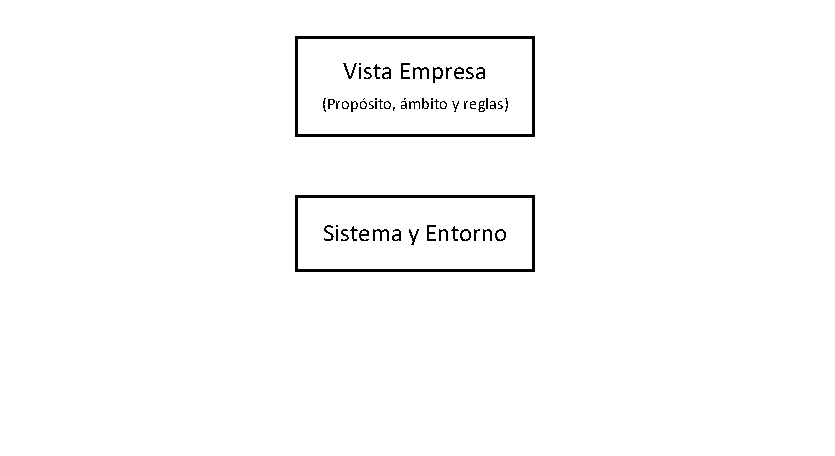
\includegraphics[width=11cm,keepaspectratio=true]{images/architecturalViews/odp01.eps}}
	}
	\only<3|handout:0>{
	   \rput[lt](0.5,0){
	   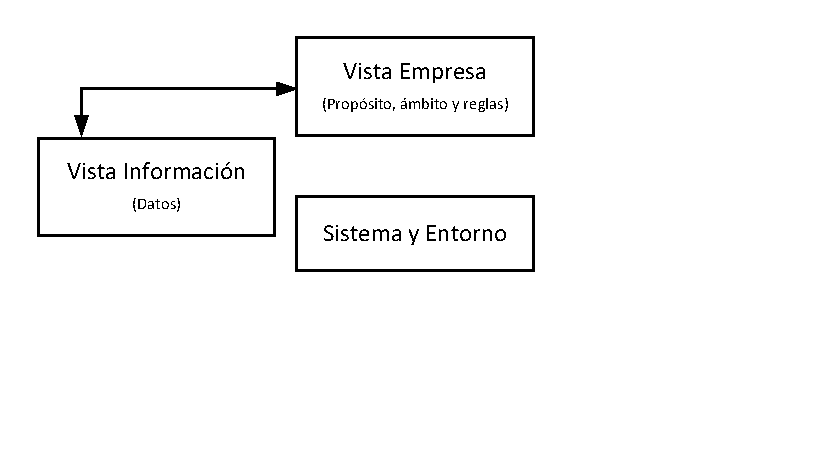
\includegraphics[width=11cm,keepaspectratio=true]{images/architecturalViews/odp02.eps}}
	}
	\only<4|handout:0>{
	   \rput[lt](0.5,0){
	   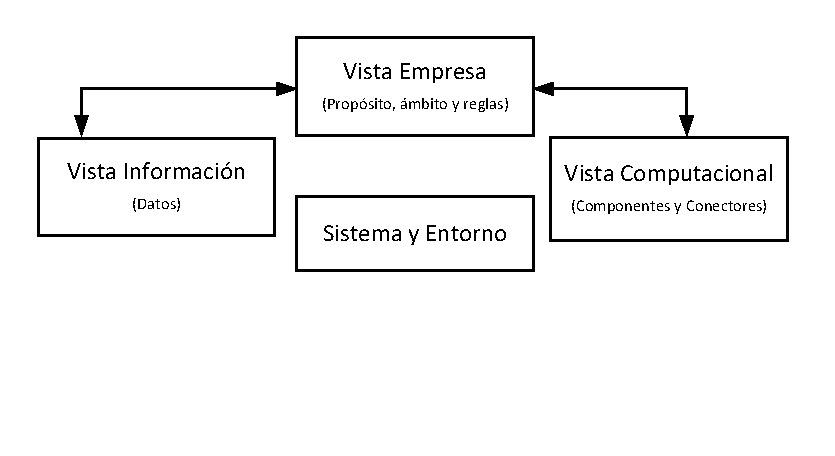
\includegraphics[width=11cm,keepaspectratio=true]{images/architecturalViews/odp03.eps}}
	}
	\only<5|handout:0>{
	   \rput[lt](0.5,0){
	   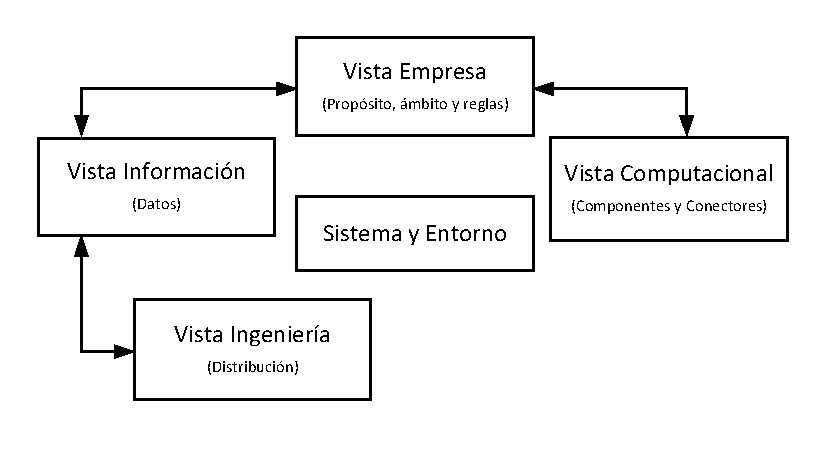
\includegraphics[width=11cm,keepaspectratio=true]{images/architecturalViews/odp04.eps}}
	}
	\only<6|handout:1>{
	   \rput[lt](0.5,0){
	   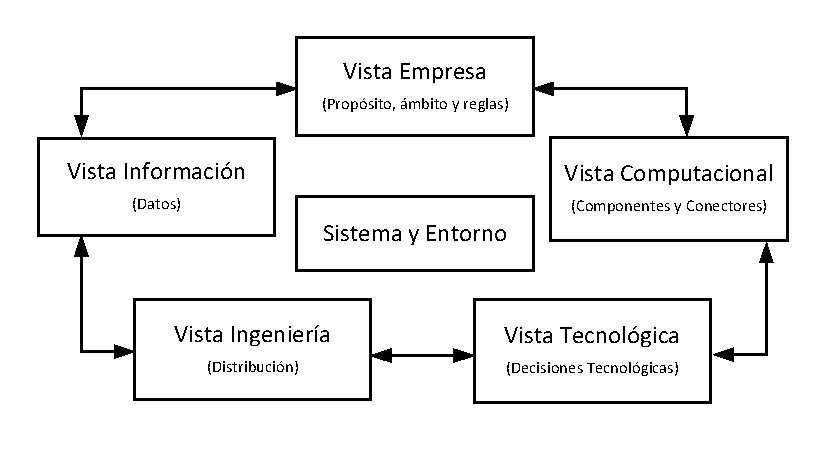
\includegraphics[width=11cm,keepaspectratio=true]{images/architecturalViews/odp05.eps}}
	}
\end{frame}

\subsection{TOGAF}

\begin{frame}
	\frametitle{TOGAF}
	%% Arquitectura empresarial del open group
	\only<1|handout:0>{
	   \rput[lt](0.5,0){
	   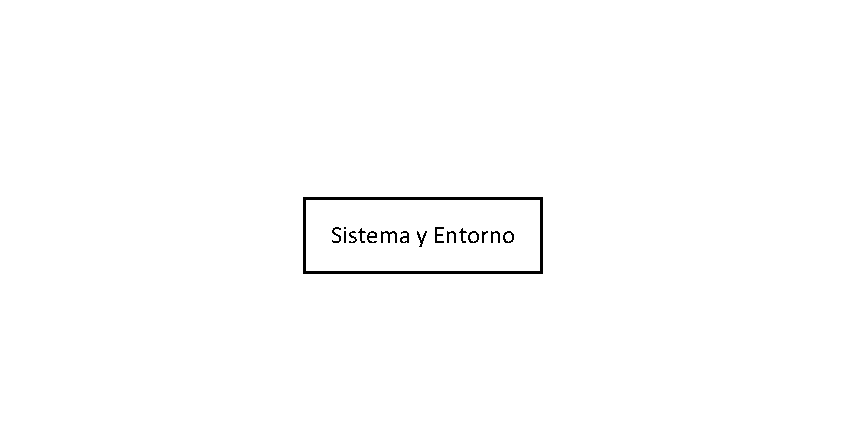
\includegraphics[width=11cm,keepaspectratio=true]{images/architecturalViews/togaf00.eps}}
	}
	\only<2|handout:0>{
	   \rput[lt](0.5,0){
	   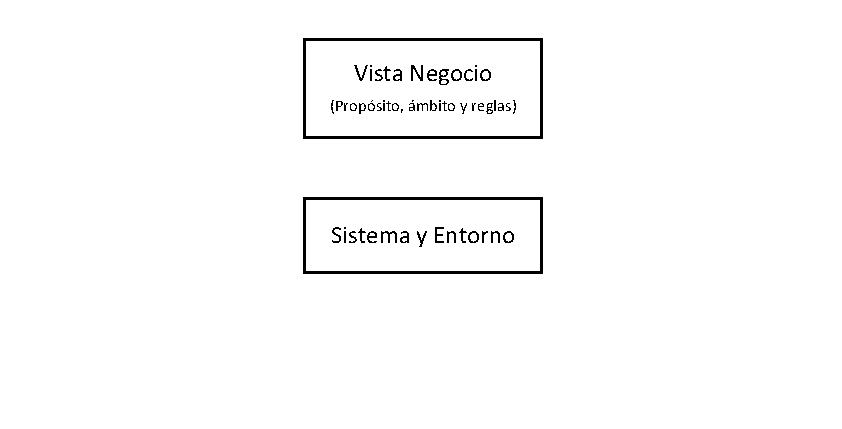
\includegraphics[width=11cm,keepaspectratio=true]{images/architecturalViews/togaf01.eps}}
	}
	\only<3|handout:0>{
	   \rput[lt](0.5,0){
	   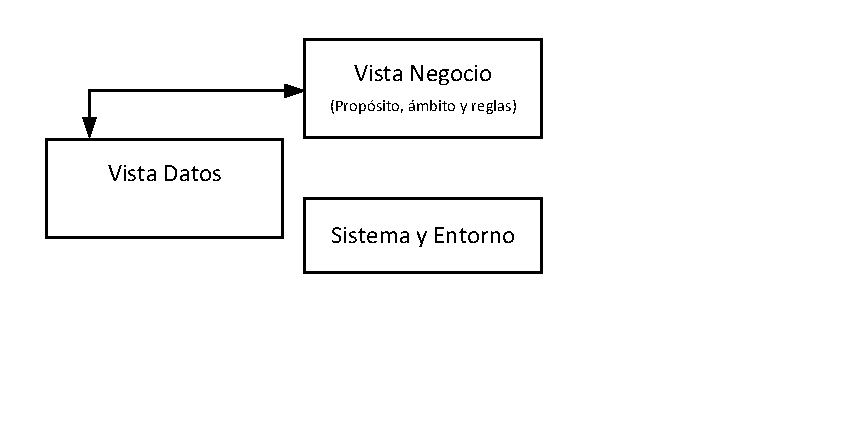
\includegraphics[width=11cm,keepaspectratio=true]{images/architecturalViews/togaf02.eps}}
	}
	\only<4|handout:0>{
	   \rput[lt](0.5,0){
	   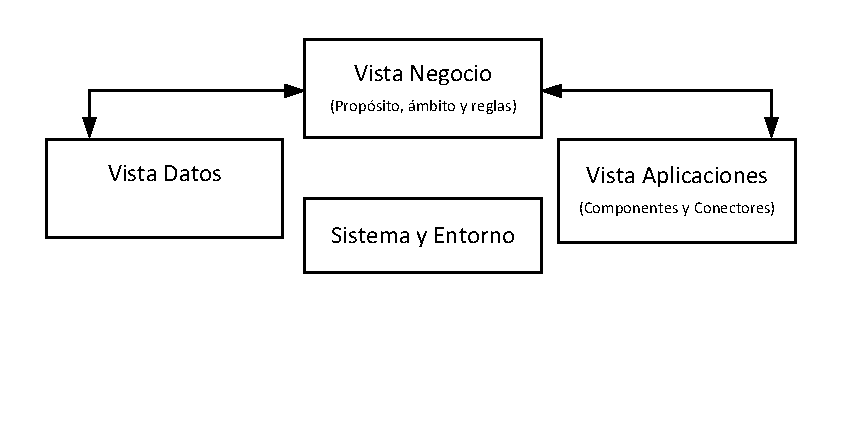
\includegraphics[width=11cm,keepaspectratio=true]{images/architecturalViews/togaf03.eps}}
	}
	\only<5|handout:1>{
	   \rput[lt](0.5,0){
	   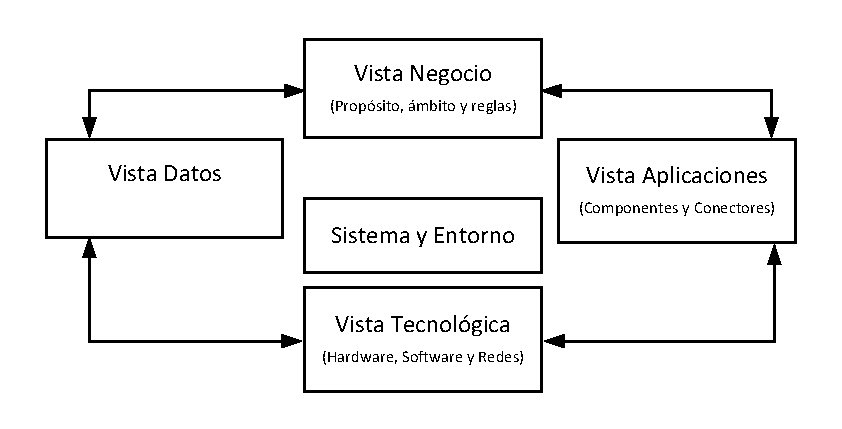
\includegraphics[width=11cm,keepaspectratio=true]{images/architecturalViews/togaf04.eps}}
	}
\end{frame}

\section{Estilos y Patrones Arquitectónicos}

\subsubsection{Introducción}

\begin{frame}
	\frametitle{Estilos y Patrones Arquitectónicos}
	\begin{block}{Estilo Arquitectónico}
		Un \emph{estilo arquitectónico} es un conjunto con nombre de decisiones de diseño que:
		\begin{enumerate}[<+->]
			\item Son aplicables dentro de un contexto determinado;
			\item Restringen las decisiones arquitectónicas dentro de dicho contexto para un sistema concreto;
			\item Pone de manifiesto las bondades de cada sistema concreto.
		\end{enumerate}
		%% Client-server
	\end{block}
	\uncover<4->{
		\begin{block}{Patrón Arquitectónico}
			Un \emph{patrón arquitectónico} es un conjunto con nombre de decisiones de diseño reutilizables que son aplicables a problemas de diseño arquitectónico recurrentes y que necesitan ser instanciadas antes de ser aplicadas a un sistema concreto.
		\end{block}
	}
	%% Diferencias entre estilo y patrón:
	%% - Estilo se aplica a un contexto o tipo de sistema (sistemas distribuidos),
	%%   mientras que el patrón se aplica a un tipo de problema (varias vistas)
	%% - Un estilo impone restricciones, mientras que un patrón aporta soluciones
\end{frame}

\subsection{Arquitecturas en Capas}

\begin{frame}[c]
	\frametitle{Arquitecturas en Capas}
	\begin{center}
		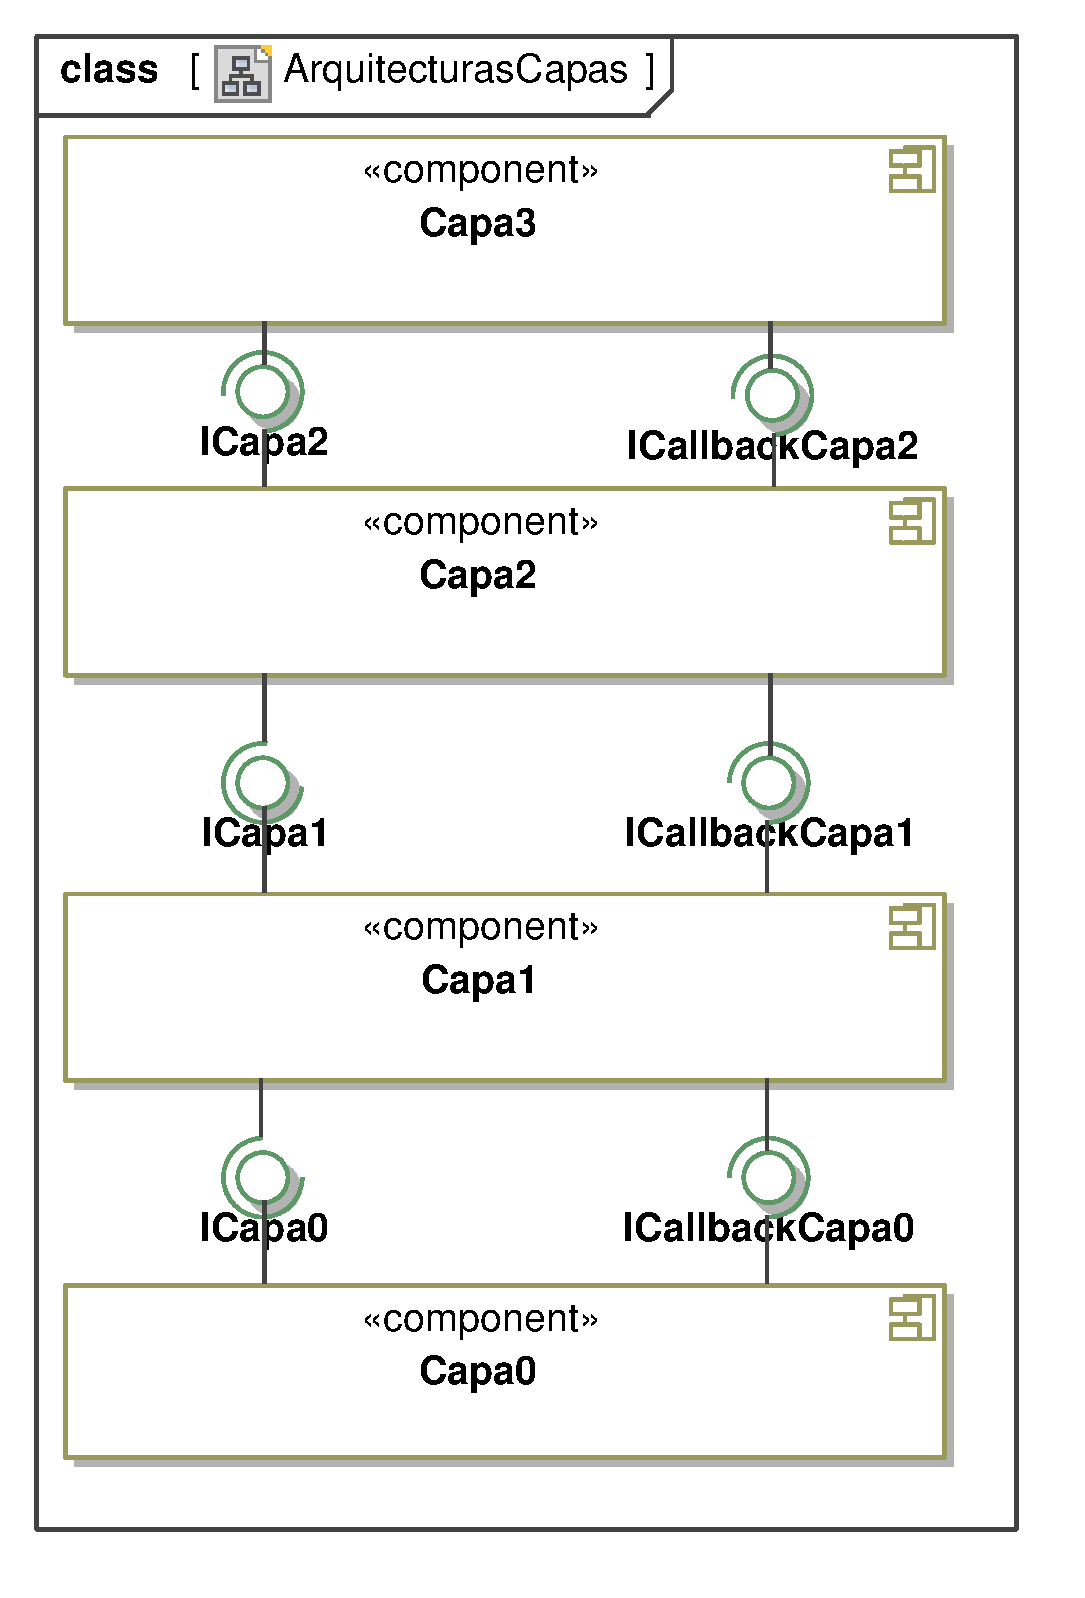
\includegraphics[width=.40\linewidth,keepaspectratio=true]{images/patterns/layered00.eps}
	\end{center}
\end{frame}

\begin{frame}[c]
	\frametitle{Arquitecturas en Capas}
	\begin{center}
		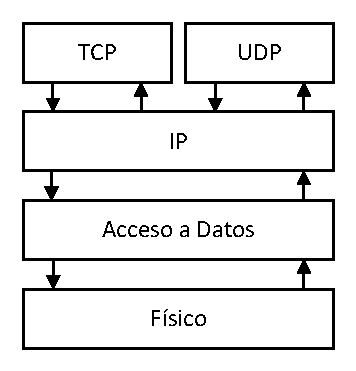
\includegraphics[width=.5\linewidth,keepaspectratio=true]{images/patterns/layered01.eps}
	\end{center}
\end{frame}

%\begin{frame}[c]
%	\frametitle{Arquitecturas en Capas}
%	\begin{center}\textbf{Ventajas}\end{center}
%	\begin{enumerate}
%		\item<2-> Independencia entre capas.
%		\item<3-> Mayor estabilidad del diseño en relación a la evolución de cada capa.
%		\item<4-> Proporciona mejores niveles de abstracción.
%	\end{enumerate}
%\end{frame}

\subsection{Arquitectura Basada en Tuberías y Filtros}

\begin{frame}[c]
	\frametitle{Arquitectura Basada en Tuberías y Filtros}
	\begin{center}
		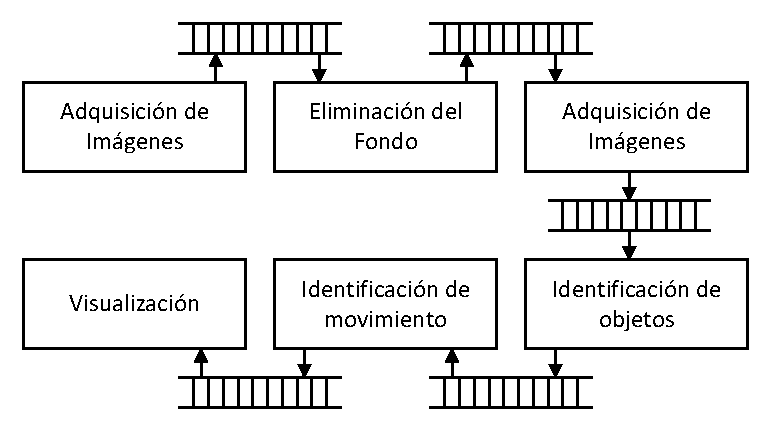
\includegraphics[width=\linewidth,keepaspectratio=true]{images/patterns/pipesFilters.eps}
	\end{center}
\end{frame}

%% Ejemplo actual: Map Reduce

\subsection{Arquitecturas basadas en Publicación/Suscripción}

\begin{frame}[c]
	\frametitle{Arquitecturas basadas en Publicación/Suscripción}
	\begin{center}
		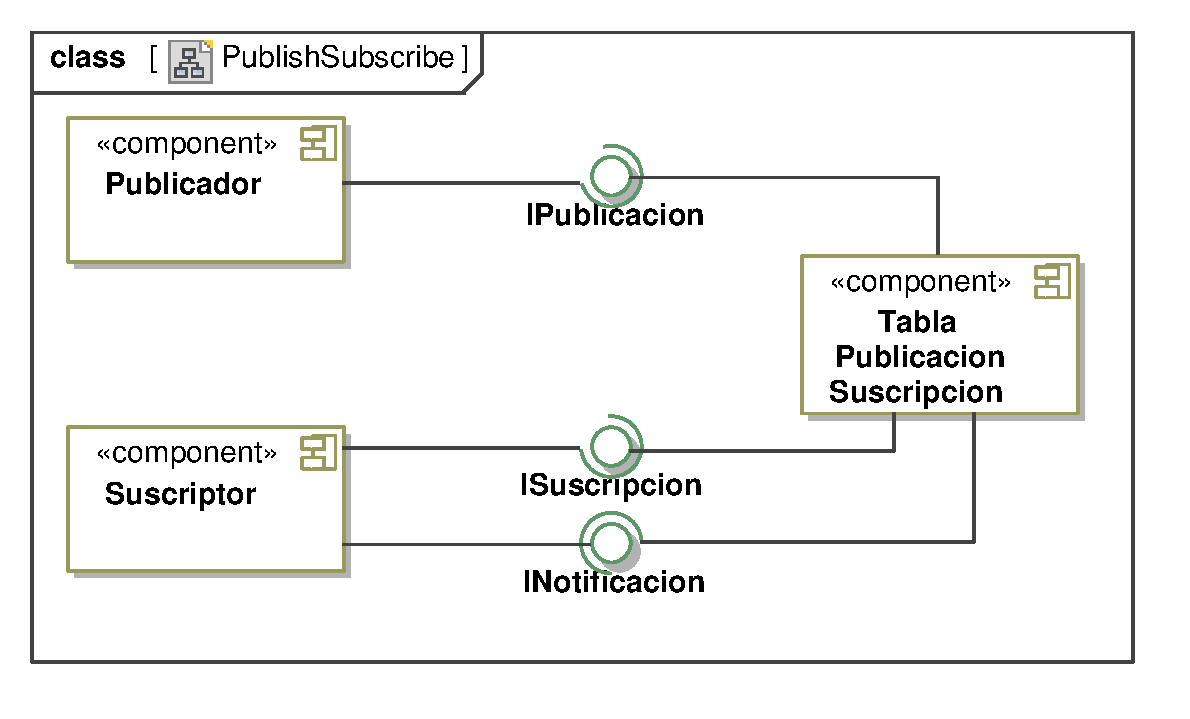
\includegraphics[width=.85\linewidth,keepaspectratio=true]{images/patterns/publishSubscribe00.eps}
	\end{center}
\end{frame}

\begin{frame}[c]
	\frametitle{Arquitecturas basadas en Publicación/Suscripción}
	\begin{center}
		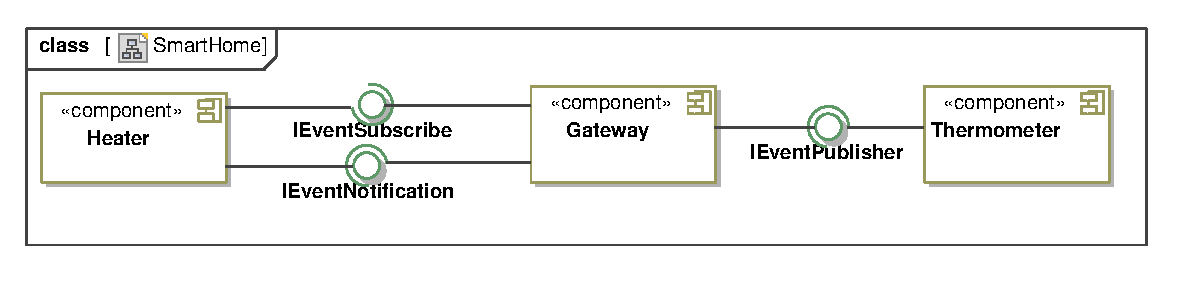
\includegraphics[width=\linewidth,keepaspectratio=true]{images/patterns/publishSubscribe01.eps}
	\end{center}
\end{frame}

\begin{frame}[t]
	\frametitle{Arquitecturas basadas en Publicación/Suscripción}
    \only<1|handout:0>{
       \rput[lt](-0.25,-1){
       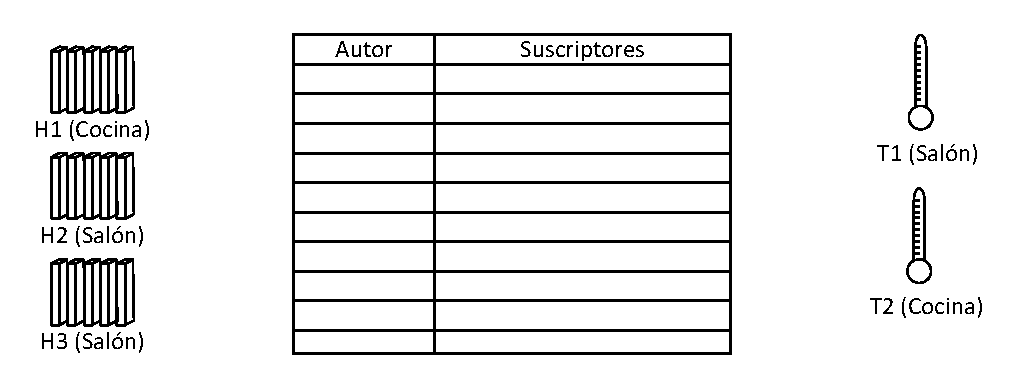
\includegraphics[width=\linewidth,keepaspectratio=true]{images/patterns/psExample00.eps}}
    }
    \only<2|handout:0>{
       \rput[lt](-0.25,-1){
       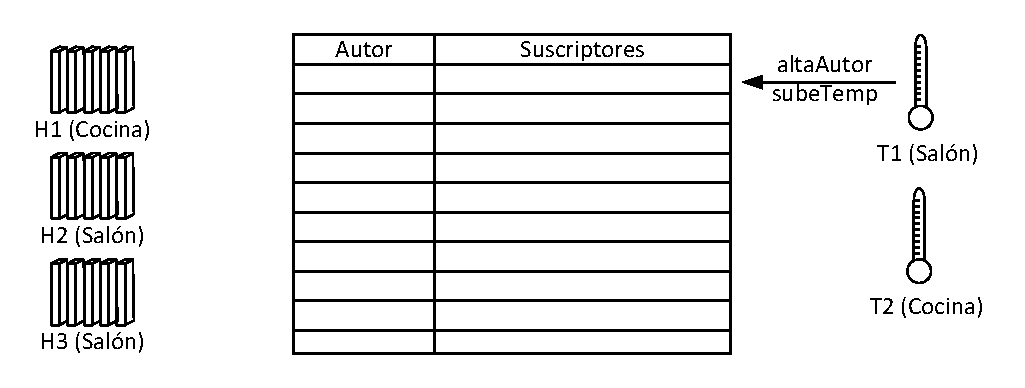
\includegraphics[width=\linewidth,keepaspectratio=true]{images/patterns/psExample01.eps}}
    }
    \only<3|handout:0>{
       \rput[lt](-0.25,-1){
       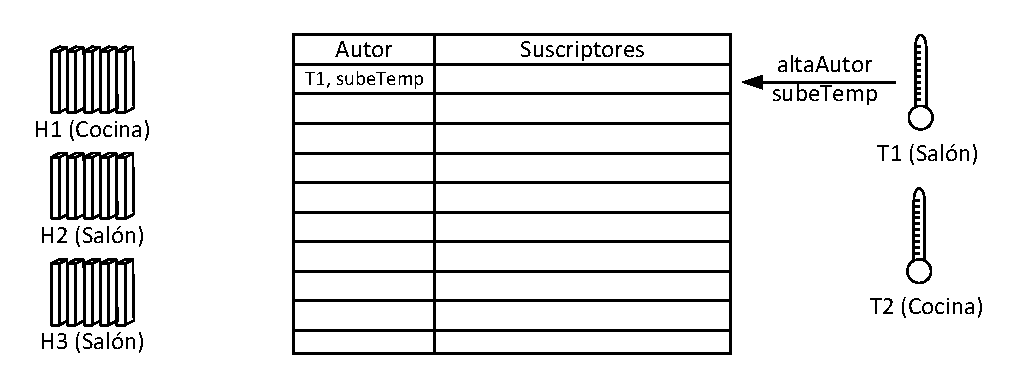
\includegraphics[width=\linewidth,keepaspectratio=true]{images/patterns/psExample02.eps}}
    }
    \only<4|handout:0>{
       \rput[lt](-0.25,-1){
       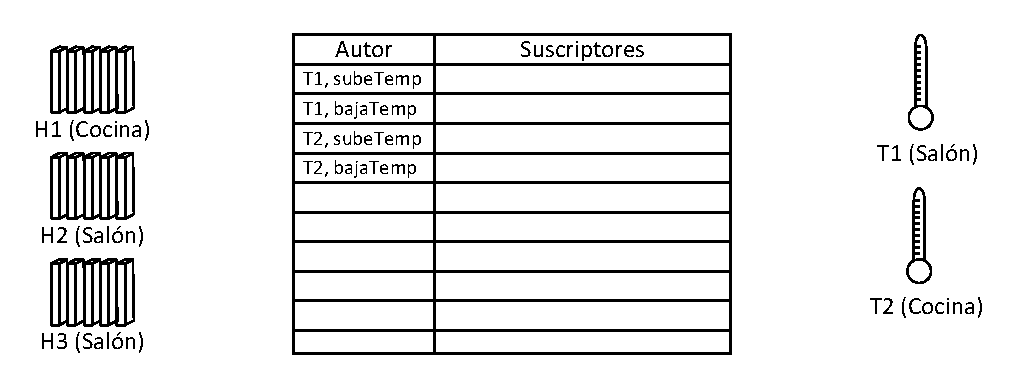
\includegraphics[width=\linewidth,keepaspectratio=true]{images/patterns/psExample03.eps}}
    }
    \only<5|handout:0>{
       \rput[lt](-0.25,-1){
       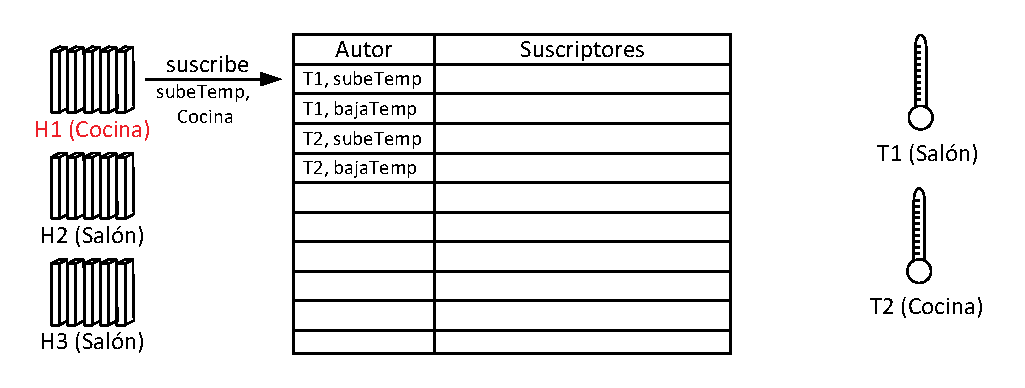
\includegraphics[width=\linewidth,keepaspectratio=true]{images/patterns/psExample04.eps}}
    }
    \only<6|handout:0>{
       \rput[lt](-0.25,-1){
       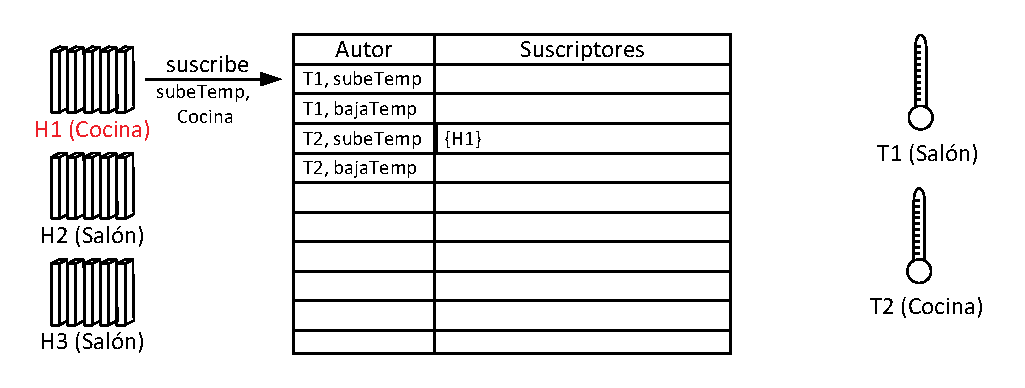
\includegraphics[width=\linewidth,keepaspectratio=true]{images/patterns/psExample05.eps}}
    }
    \only<7|handout:0>{
       \rput[lt](-0.25,-1){
       \includegraphics[width=\linewidth,keepaspectratio=true]{images/patterns/psExample06.eps}}
    }
    \only<8|handout:0>{
       \rput[lt](-0.25,-1){
       \includegraphics[width=\linewidth,keepaspectratio=true]{images/patterns/psExample07.eps}}
    }
    \only<9|handout:0>{
       \rput[lt](-0.25,-1){
       \includegraphics[width=\linewidth,keepaspectratio=true]{images/patterns/psExample08.eps}}
    }
    \only<10|handout:0>{
       \rput[lt](-0.25,-1){
       \includegraphics[width=\linewidth,keepaspectratio=true]{images/patterns/psExample09.eps}}
    }
    \only<11|handout:0>{
       \rput[lt](-0.25,-1){
       \includegraphics[width=\linewidth,keepaspectratio=true]{images/patterns/psExample10.eps}}
    }
    \only<12|handout:0>{
       \rput[lt](-0.25,-1){
       \includegraphics[width=\linewidth,keepaspectratio=true]{images/patterns/psExample11.eps}}
    }
	\only<13|handout:1>{
	   \rput[lt](-0.25,-1){
	   \includegraphics[width=\linewidth,keepaspectratio=true]{images/patterns/psExample12.eps}}
	}
\end{frame}

%%============================================================================================%%
%% Ventajas: 	                                                                              %%
%% * Publicadores y suscriptores desacoplados.                                                %%
%% * Vinculación suscriptor-publicador dinámica.                                              %%
%%============================================================================================%%

\section{Proceso de Diseño de Arquitecturas}

%\subsection{El Modelo de Desarrollo en Turbina}
%
%\begin{frame}[c]
%	\frametitle{Modelo de Desarrollo en Turbina~\cite{taylor:2009}}
%	\begin{center}
%		\includegraphics[width=.9\linewidth]{images/disenho/turbina00.eps}
%	\end{center}
%\end{frame}
%
%\begin{frame}[c]
%	\frametitle{Modelo de Desarrollo en Turbina}
%	\begin{center}
%		\includegraphics[width=.9\linewidth]{images/disenho/turbina01.eps}
%	\end{center}
%\end{frame}
%
%\begin{frame}[c]
%	\frametitle{Modelo de Desarrollo en Turbina}
%	\begin{center}
%		\includegraphics[width=.60\linewidth]{images/disenho/turbina02.eps}
%	\end{center}
%\end{frame}

% \subsection{Consejos sobre Diseño de Arquitecturas}

\begin{frame}[c]
	\frametitle{Consejos sobre Diseño de Arquitecturas}
	\begin{enumerate}
		\item<1-> Seleccionar estilo o patrón arquitectónico a aplicar.
		\item<2-> Definir los principios o reglas generales de diseño (textura).
		\item<3-> Crear una primera estructura básica.
		\item<4-> Analizar dicha estructura básica.
		\item<5-> Planificar estrategias satisfacción requisitos no funcionales.
		\item<6-> Por cada caso de uso, asignar responsabilidades a las interfaces de los componentes. \uncover<7->{Opcional: Crear un escenario arquitectónico que indique como se satisface cada caso de uso}.
		\item<8-> Identificar topología de red y asignar componentes a nodos.
	\end{enumerate}
\end{frame}

%% \subsection{Attribute-Driven Design (AAD)}

%% \subsection{Diseño de Requisitos No Funcionales}

%\begin{frame}[c]
%	\frametitle{Diseño de Requisitos No Funcionales}
%	\begin{description}
%		\item<+->[Eficiencia] Planificadores, cachés, replicación y balanceo de carga.
%		\item<+->[Portabilidad] Middleware portable, estándares de comunicación,
%		\item<+->[Tolerancia a fallos] Transacciones, integridad mensajes, réplicas.
%	\end{description}
%\end{frame}
%
%\begin{frame}[c]
%	\frametitle{Diseño de Arquitecturas Seguras}
%	%%==============================================================================%%
%	%% NOTA(Pablo) : Esto es mejor hablarlo con Carlos                              %%
%	%%==============================================================================%%
%	\begin{block}{Seguridad}
%		Capacidad de un sistema de mantener la \alert<2->{\emph{integridad}}, \alert<3->{\emph{disponibilidad}} y \alert<4->{\emph{confidencialidad}} de sus recursos.
%	\end{block}
%	\uncover<5->{
%		\begin{block}{Confidencialidad}
%			Prevenir el acceso no autorizado a cierta información o incluso evitar que entidades no autorizadas puedan saber que cierta información sensible existe.
%		\end{block}
%	}
%	\uncover<6->{
%		\begin{block}{Integridad}
%			Sólo las entidades autorizadas deben ser capaces de modificar el sistema.
%		\end{block}
%	}
%	\uncover<7->{
%		\begin{block}{Disponibilidad}
%			Las entidades deben tener siempre acceso a los recursos autorizados.
%		\end{block}
%	}
%\end{frame}
%
%\begin{frame}[c]
%	\frametitle{Seguridad basada en Control de Accesos}
%	\begin{center}
%		\includegraphics[width=\linewidth]{images/disenho/security00.eps}
%	\end{center}
%\end{frame}
%
%\begin{frame}[c]
%	\frametitle{Seguridad basada en Control de Accesos}
%	\begin{center}
%		\includegraphics[width=\linewidth]{images/disenho/security01.eps}
%	\end{center}
%\end{frame}
%
%\begin{frame}[c]
%	\frametitle{Seguridad}
%	\begin{description}
%		\item<+->[Subject] Entidad (software o física) que intenta acceder a un recurso protegido, y que puede poseer atributos.
%		%% Student, teacher
%		\item<+->[Resource/Object] Entidad (dato o servicio) cuyo acceso hay que proteger.
%		%% A data, an operation
%		\item<+->[Principal] Credenciales que un objeto posee para obtener un cierto permiso.
%		%% A teacher is student and teacher
%		\item<+->[Permission] Operaciones que se pueden ejecutar sobre un objeto o recurso.
%		%% Invoke, Write, Read
%		\item<+->[Privilege] Permisos que posee un sujeto de acuerdo a sus credenciales.
%		%% A teacher can invoke operations
%		\item<+->[Safeguard] Permisos que son necesarios para acceder a un recurso.
%		%% A student cannot change its calification
%		\item<+->[Policy] Reglas que especifican qué privilegios debe poseer un sujeto, de acuerdo a su conjunto de credenciales, para poder acceder a un recurso protegido mediante una cierta guarda de seguridad.
%	\end{description}
%\end{frame}
%
%\begin{frame}[c]
%	\frametitle{Listas de Control de Accesos}
%	\begin{center}
%	\begin{tabular}{||l|c|c||}
%	   \hline \hline
%								  & Auction System & Store Clerk \\ \hline
%	   \texttt{assignOrder}       &   No           &   Yes       \\ \hline
%	   \texttt{changeOrderStatus} &   No           &   Yes       \\ \hline
%	   \texttt{pickOrder}         &   Yes          &   No        \\ \hline
%	   \texttt{sendOrder}         &   Yes          &   No        \\ \hline
%	   \texttt{viewOrders}        &   No           &   Yes       \\
%	   \hline \hline
%	\end{tabular}
%	\end{center}
%\end{frame}

\section{Análisis de Arquitecturas}

\subsection{Introducción}

\begin{frame}[c]
	\frametitle{Análisis Arquitectónico}
	\begin{block}{Análisis Arquitectónico}
		Proceso por el cual se descubren y verifican propiedades importantes de un sistema a partir de sus
		modelos arquitectónicos.
	\end{block}
	\uncover<2->{
	\begin{block}{Objetivos del análisis}
	\begin{enumerate}
		\item<3-> Completitud.
		\item<4-> Consistencia.
		\item<5-> Compatibilidad.
		%% Estándares
		\item<6-> Corrección.
	\end{enumerate}
	\end{block}
	}
\end{frame}

%\subsection{Matrices de trazabilidad}
%
%\begin{frame}[c]
%	\frametitle{Matrices de trazabilidad}
%	   \begin{center}\begin{small}
%	   \begin{tabular}{||l|c|c|c|c||}
%	   \hline \hline            & \texttt{AuctionSystem} & \texttt{SellerUI} & \texttt{BuyerUI} &  \texttt{Database} \\ \hline
%	   \texttt{Create Auction}  &          X             &         X         &                  &          X         \\ \hline
%	   \texttt{Close Auction}   &          X             &                   &                  &          X         \\ \hline
%	   \texttt{Propose Bid}     &          X             &                   &        X         &          X         \\ \hline
%	   \texttt{Start Auction}   &          X             &                   &                  &          X         \\ \hline
%	   \hline
%	\end{tabular}
%	\end{small}\end{center}
%\end{frame}

\subsection{ATAM}

\begin{frame}[c]
	\frametitle{Architectural Trade-Off Analysis Method (ATAM)}
	\begin{center}
	  \includegraphics[width=\linewidth]{images/analysis/atam.eps}
	\end{center}
	%% The purpose of the ATAM is to assess the consequences of architectural
	%% decisions in light of quality attribute requirements.

	%% Sensitivity points are parameters in the architecture to which some measurable
	%% quality attribute response is highly correlated.

	%% This is achieved in part by eliciting scenarios from the stakeholders that
	%% clearly state the quality attribute requirements in terms of stimuli and responses
\end{frame}

\begin{frame}[c]
	\frametitle{Architectural Trade-Off Analysis Method (ATAM)}
	\begin{enumerate}
		\item<+-> Explicar ATAM a los diferentes actores involucrados en el proceso.
		\item<+-> Presentar las características fundamentales del productos.
		\item<+-> Explicar la arquitectura propuesta.
		\item<+-> Explicar estilos y patrones arquitectónicos aplicados.
		\item<+-> Crear un árbol de de escenarios resaltando atributos de calidad que deben satisfacerse.
		\item<+-> Analizar cómo los estilos y patrones arquitectónicos satisfacen los atributos de calidad.
		\item<+-> Identificación y priorización de nuevos escenarios.
		\item<+-> Analizar cómo los estilos y patrones arquitectónicos satisfacen los atributos de calidad.
		\item<+-> Presentar los resultados.
	\end{enumerate}
\end{frame}

\begin{frame}[c]
	\frametitle{Escenarios ATAM}
	\begin{description}
		\item<+->[Casos de Uso] Operaciones de usuario
		\item<+->[Crecimiento] Gestión de cambios anticipados.
		\item<+->[Exploratorios]  Gestión de cambios no anticipados y drásticos.
	\end{description}
\end{frame}

%% Añadir una gráfico de ATAM

\section{Sumario y Referencias}

\subsection{Sumario}

\begin{frame}[c]
	\frametitle{¿Qué tengo que saber de todo esto?}
	\begin{enumerate}[<+->]
		\item Comprender el concepto de arquitectura software,.
		\item Comprender el concepto de vista arquitectónica.
		\item Conocer las vistas arquitectónicas más comunmente utilizadas.
		\item Conocer las vistas utilizadas por algún modelo arquitectónico de referencia como \emph{TOGAF}.
		% \item Conocer alguna metodología de diseño de arquitecturas como AAD.
        \item Conocer algunas directrices para el diseño de arquitecturas sw.
        \item Conocer alguna metodología de análisis de arquitectura como ATAM.
        \item Conocer algunos patrones arquitectónicos de dominios diferentes a las arquitecturas empresariales.
	\end{enumerate}
\end{frame}

\subsection{Referencias}

\begin{frame}[allowframebreaks]
	\frametitle{Referencias}
	\bibliographystyle{apalike}
	\bibliography{disenhoSoftware}
\end{frame}

\end{document}
